\documentclass{article}
\usepackage[utf8]{inputenc}
\usepackage[T1]{fontenc}
\usepackage[german]{babel}
\usepackage{amsmath}
\usepackage{amsthm}
\usepackage{amsfonts}
\usepackage{amssymb}
\usepackage{minted}
\usepackage{tikz}
\usepackage{pgfplots}
\usepackage[top=2cm, bottom=2cm, left=2cm, right=2cm, headheight=1.5cm]{geometry}
\usepackage{fancyhdr}
\usepackage{mdframed}
\usemintedstyle{emacs}

\definecolor{purp}{HTML}{9A72AC}
\definecolor{re}{HTML}{FC6255}
\definecolor{gre}{HTML}{83C167}
\definecolor{blu}{HTML}{58C4DD}
\definecolor{shadecolor}{rgb}{0.85,0.85,0.85}
\definecolor{bg}{rgb}{0.95,0.95,0.95}
\setlength{\parindent}{0em} 

\BeforeBeginEnvironment{minted}{\begin{mdframed}[linewidth =2 ,backgroundcolor=bg , linecolor=black, linewidth=0.5]}
\AfterEndEnvironment{minted}{\end{mdframed}}

\newenvironment{defi}[1]{
    \begin{shaded*}
    \textbf{Definition #1} \\
}{
    \end{shaded*}
}

\newcommand{\bsp}{\textbf{Beispiel}:}
%\newcommand{\task}{\textbf{Aufgabe}:}

\newcommand{\bol}[1]{\textbf{#1}}
\newcommand{\q}[1]{\glqq #1\grqq}
\newcommand{\DODO}[1]{\textbf{\textcolor{red}{DODO:}} #1 \\ \begin{center}\includegraphics[scale=0.2]{../../media/dodo.jpg} \end{center}}

\newenvironment{task}[1]{
    \begin{shaded*}
    \textbf{Aufgabe #1}:
}{
    \end{shaded*}
}



\fancypagestyle{firstpage}{
    \setlength{\headheight}{2.5cm}
    \setlength{\footskip}{0.25cm}
    \pagestyle{fancy}
    \renewcommand{\headrulewidth}{0.4pt}
    \fancyhf{}
    \fancyhead[L]{\LARGE\textbf{Musterlösung und Erläuterungen S. 216|2}}
    \fancyfoot[C]{\thepage}
}
\begin{document}
\thispagestyle{firstpage}
\setlength{\headsep}{12pt}
Aufgabentext:
\begin{center}
    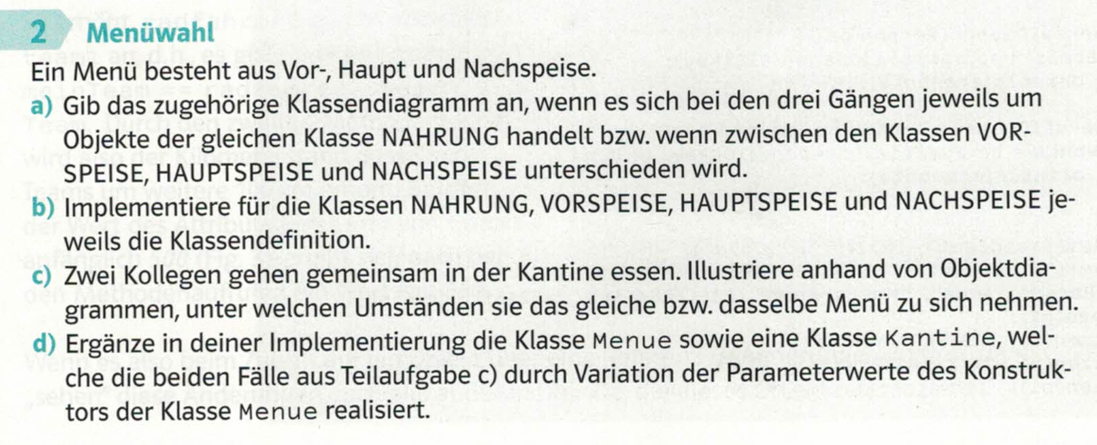
\includegraphics[scale=0.6]{media/216_2.png}
\end{center}
\textbf{a) und b)} In jedem der angesprochenen Fälle brauchen wir eine Klasse Menü, es ändern sich lediglich die Referenzen auf die entsprechenden Vorspeisen, Hauptgerichte bzw. Nachspeisen. Die zusätzlichen Attribute bzw. Methoden sind nicht von der Aufgabe vorgegeben, dienen aber der weiteren Veranschaulichung der Situation. \\
\textbf{Achtung:} Die Attribute, die Referenzen auf Objekte anderer Klassen darstellen (im ersten Fall z.B. auf Objekte der Klasse Nahrung), werden üblicherweise nicht mehr explizit im Klassendiagramm angegeben (anders als im Buch auf S. 209 z.B.), da diese Information bereits in der Verbindungslinie steckt (eine zusätzliche Angabe ist in diesem Sinne aber nicht falsch, nur unnötig, da doppelte Information abgebildet wird).
\textbf{Erster Fall:}
\begin{center}
    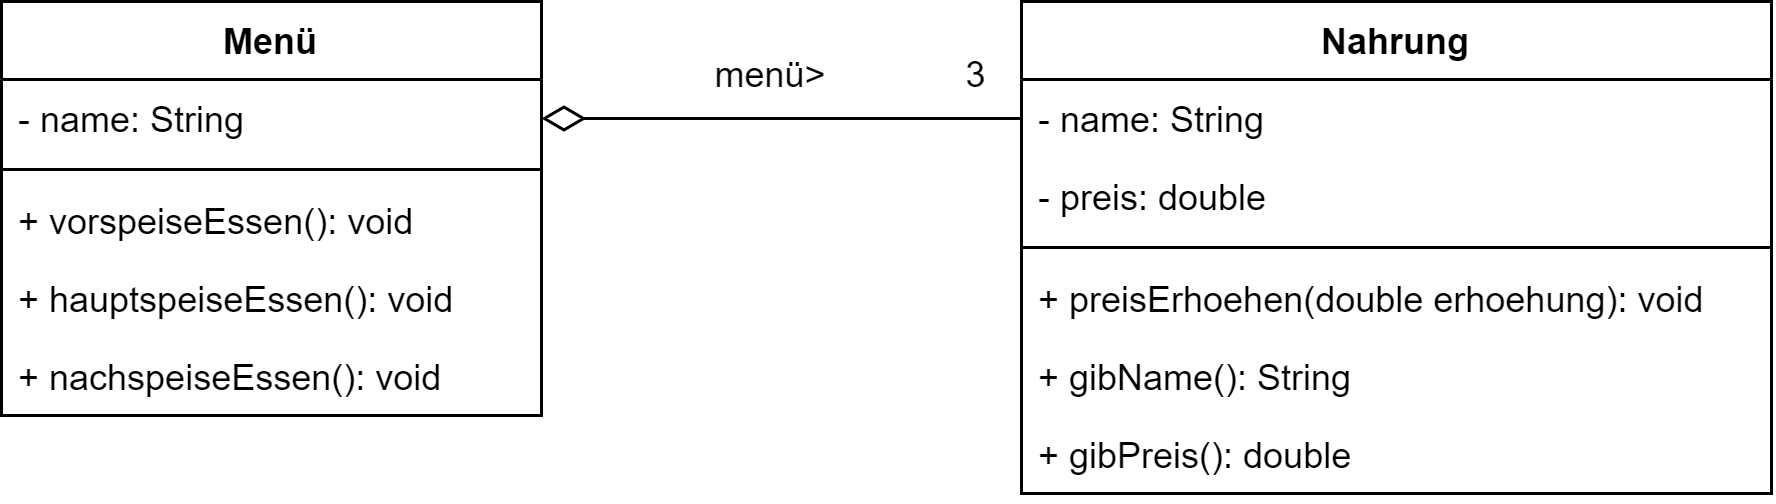
\includegraphics[scale=0.25]{media/menue_nahrung.png}
\end{center}
Wenn man sich das Klassendiagramm ansieht - und die Aufgabe vorher nicht liest - würde man schlussfolgern, dass ein Menü drei Objekte vom Typ Nahrung enthält. Es wird dabei keine Vorgabe gemacht, wie diese Referenzen auf die Nahrungsobjekte gespeichert werden! Man könnte hier z.B. implementieren:
\begin{minted}{java}
public class Menü {
    private Nahrung vorspeise;
    private Nahrung hauptgericht;
    private Nahrung nachspeise;

    public Menü() {
        vorspeise = new Nahrung(...);
        hauptgericht = new Nahrung(...);
        nachspeise = new Nahrung(...);
    }
}
\end{minted}
Der entsprechende Konstruktor für Nahrung muss natürlich noch definiert werden. Alternativ könnte man die drei Teile des Menüs aber auch in einem Feld speichern:
\begin{minted}{java}
public class Menü {
    private Nahrung[] menü;

    public Menü() {
        menü = new Nahrung[3];
        menü[0] = new Nahrung(...) // Vorspeise
        menü[1] = new Nahrung(...) // Hauptspeise
        menü[2] = new Nahrung(...) // Nachspeise
    }
}
\end{minted}
Die zweite verlangte Variante legt die Verwendung einer Oberklasse nahe, da Methoden wie preisErhöhen() oder auch gibName()  natürlich für alle Speisen sinnvoll sind (für dieses minimale Beispiel ist natürlich fraglich, ob wir wirklich Unterklassen brauchen, in der \q{Realität} sicher nicht!), deswegen ergibt sich folgendes Klassendiagramm:
\begin{center}
    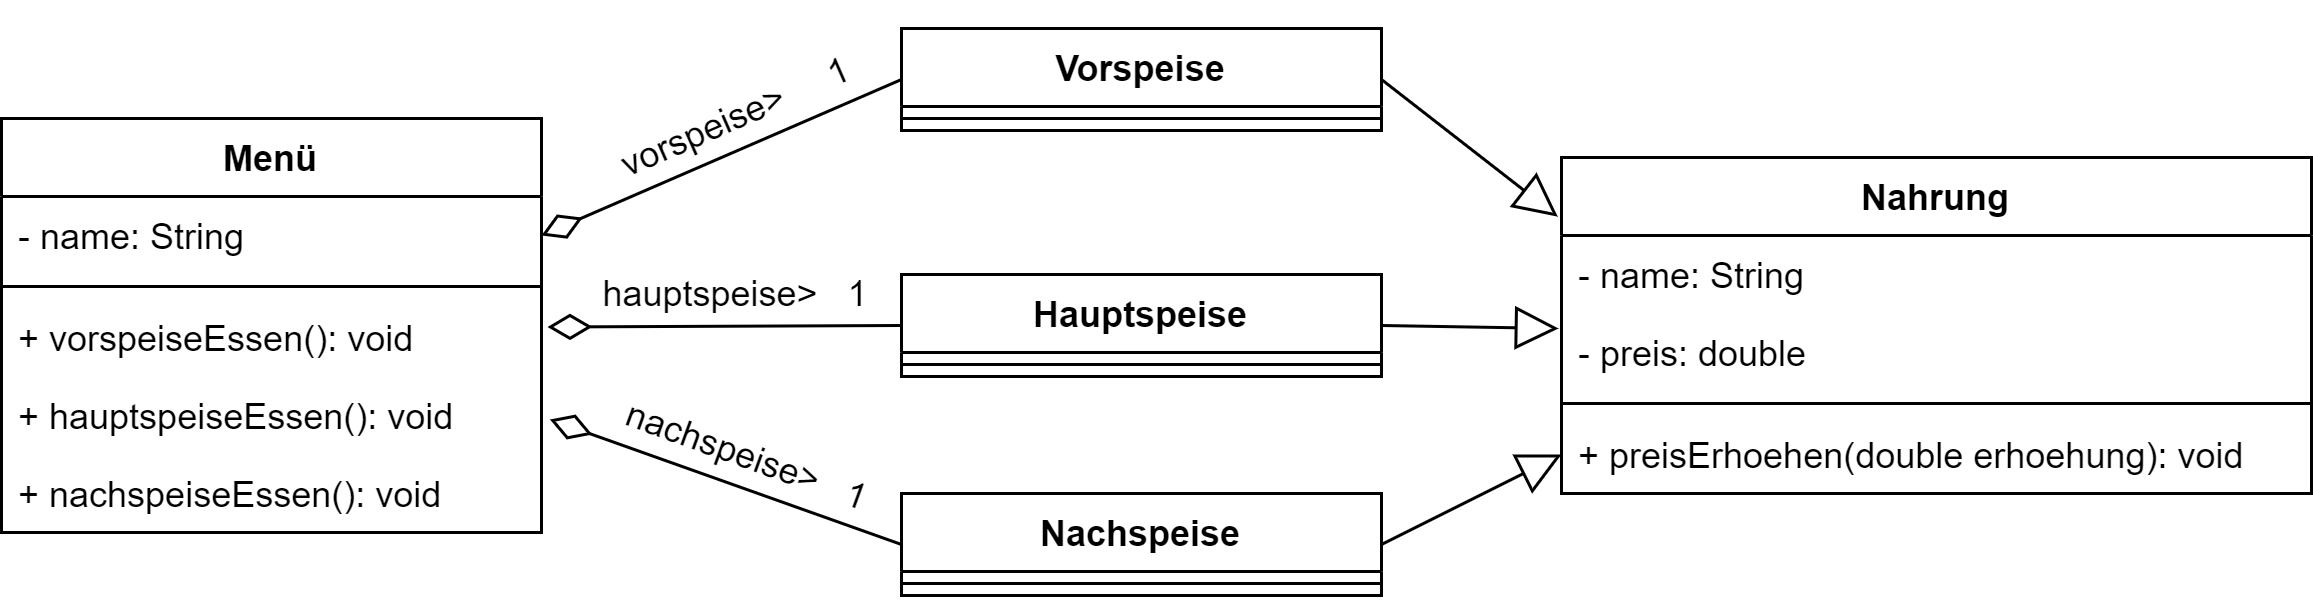
\includegraphics[scale=0.2]{media/menue_geteilt.png}
\end{center}
Für diese Variante sieht die Implementierung wie folgt aus (bereits mit den Zusatzmethoden für Nahrung):
\begin{minted}{java}
public class Nahrung {
     
    private String name;
    private double preis;
    
    public Nahrung(String name, double preis) {
        this.name = name;
        this.preis = preis;
    }
        
    public String gibName() {
        return name;
    }
    
    public double gibPreis() {
        return preis;
    }
    
    public void preiserhoehen(double erhoehung) {
        preis += erhoehung;
    }
}
public class Vorspeise extends Nahrung {
    
    public Vorspeise(String name, double preis) {
        super(name, preis);
    }
}
public class Hauptspeise extends Nahrung {
    
    public Hauptspeise(String name, double preis) {
        super(name, preis);        
    }
}
public class Nachspeise extends Nahrung { 
    public Nachspeise(String name, double preis) {
        super(name, preis);
    }
}
\end{minted}
\textbf{c)} Die Aufgabe spielt darauf an, dass zwei Menüs auf dasselbe oder auf unterschiedliche Objekte zeigen können, die gesuchte Veranschaulichung sieht so aus: 
\begin{center}
    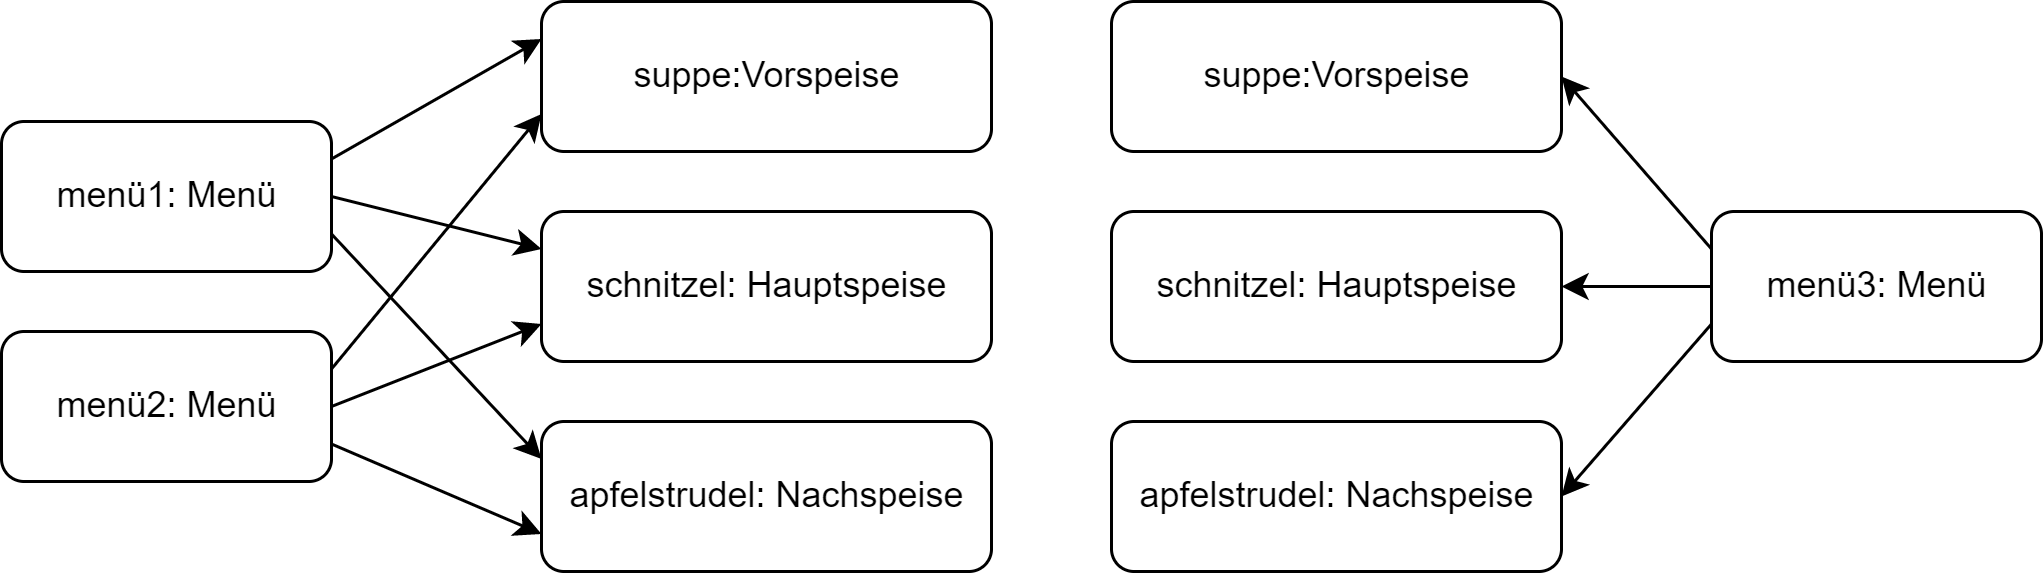
\includegraphics[scale=0.2]{media/menue_objektdiagram.png}
\end{center}
Die beiden Objekte \textbf{menü1} und \textbf{menü2} zeigen beide auf jeweils dasselbe Objekt der Klasse Vorspeise, Nachspeise und Hauptspeise. Das \textbf{menü3} zeigt zwar auf gleichartige Objekte, aber nicht auf dieselben! \\
\textbf{d)} Die ergänzten Klassen sehen z.B. so aus:
\begin{minted}{java}
    public class Menü {
    private String name;
    private Vorspeise vorspeise;
    private Hauptspeise hauptspeise;
    private Nachspeise nachspeise;
    
    public Menü(String name, Vorspeise vorspeise, Hauptspeise hauptspeise,
     Nachspeise nachspeise) {
        this.vorspeise = vorspeise;
        this.hauptspeise = hauptspeise;
        this.nachspeise = nachspeise;
        this.name = name;
    }
    
    public void vorspeiseEssen() {
        if(vorspeise != null) {
            System.out.println("lecker -  " + vorspeise.gibName());
            vorspeise = null;
        } else {
            System.out.println("Die Vorspeise wurde schon gegessen!");
        }
    }
    
    public void hauptspeiseEssen() {
        if(vorspeise != null) {
            System.out.println("lecker - " + hauptspeise.gibName());
            hauptspeise = null;
        } else {
            System.out.println("Die Hauptspeise wurde schon gegessen!");
        }
    }
    
    public void nachspeiseEssen() {
        if(vorspeise != null) {
            System.out.println("lecker - " + nachspeise.gibName());
            nachspeise = null;
        } else {
            System.out.println("Die Nachspeise wurde schon gegessen!");
        }
    }
}

public class Kantine {
    
    public Kantine() {
        Hauptspeise hauptspeise1 = new Hauptspeise("Schnitzel", 9.6);
        Hauptspeise hauptspeise2 = new Hauptspeise("Schnitzel", 9.6);
        Vorspeise vorspeise1 = new Vorspeise("Suppe", 5.2);
        Vorspeise vorspeise2 = new Vorspeise("Suppe", 5.2);
        Nachspeise nachspeise1 = new Nachspeise("Apfelstrudel", 6.10);
        Nachspeise nachspeise2 = new Nachspeise("Apfelstrudel", 6.10);
        Menü menü1 = new Menü("Super Menü", vorspeise1, hauptspeise1, nachspeise1);
        Menü menü2 = menü1;
        Menü menü3 = new Menü("Super Menü", vorspeise2, hauptspeise2, nachspeise2);
    }
}

\end{minted}

Die Essens-Methoden sind dabei natürlich nicht verlangt gewesen, waren aber im obigen Klassendiagramm erwähnt worden, deswegen ist eine Beispielimplementierung dabei. 
\end{document}